\subsection{Wheatstone Bridge} \label{ssec:BridgeCircuits}
The Wheatstone bridge has been around since the 1800 hundreds, and was among the very first methods used to characterize an unknown impedance. Originally only used for DC resistance measurements, but with a few modifications it was expanded to characterize impedances as well. 
The circuit can be seen in figure \ref{fig_4_2_WheatstoneBridge}, where $Z_1$ is the unknown device,
 often referred to as the DUT.
 
A null detector is present across the two nodes, this allows the two impedance ratios $Z_1/Z_3$ and $Z_2/Z_4$
to be matched. If there is \SI{0}{\volt} at all times across node b and d, then the ratio of $Z_1/Z_3$ will match that of
 $Z_2/Z_4$, and the
phase angle will be given as $\theta_1 - \theta_2 = \theta_2 - \theta_4$. 

\begin{figure}[H]
    \centering
    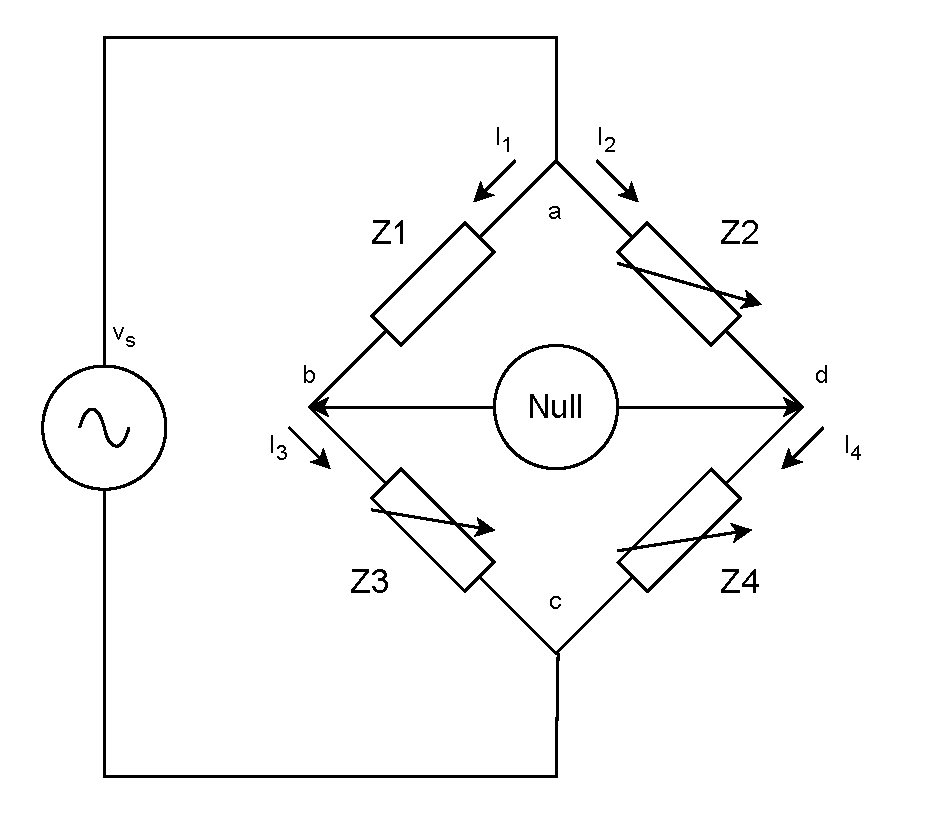
\includegraphics[width=0.75\textwidth]{Sections/4_TechnicalAnalysis/Figures_JFT/WheatstoneBridgeAC.pdf}
    \caption{A typical AC Wheatstone bridge, where Z1 is the device under test.}
    \label{fig_4_2_WheatstoneBridge}
\end{figure}

The relationship between the different impedances can be described by analyzing the bridge. The voltage across $Z_1$ and $Z_2$ can
be described as in equation \ref*{eq:4_2_TopWheatstone}.

\begin{equation}
    \begin{split}
        \label{eq:4_2_TopWheatstone}
        i_1 &= \frac{v_s-v_1}{Z_1} \Rightarrow -i_1 Z_1 +v_s = v_1 \\
        i_2 &= \frac{v_s-v_1}{Z_2} \Rightarrow -i_2 Z_2 + v_s = v_2
    \end{split}
\end{equation}

Under the assumption that the null detector reads zero, and the same voltage is present at node b and d, then the voltage
across $Z_1$ must be equal to that across $Z_2$. From this equation \ref{eq:4_2_TopWheatStone2} can be constructed, showing the
relationship between currents and impedances for the top most resistors of the bridge.

\begin{equation}
    \begin{split}
        \label{eq:4_2_TopWheatStone2}
        v_1 &= v_2 \Rightarrow -i_1 Z_1 +v_s = -i_2 Z_2 + v_s \\
        i_1 Z_1 &= i_2 Z_2 \Rightarrow \frac{i_2}{i_1} = \frac{Z_1}{Z_2}
    \end{split}
\end{equation}

In much the same way, the lower half of the bridge can be described as seen in equation \ref{eq:4_2_BotWheatstone}

\begin{equation}
    \label{eq:4_2_BotWheatstone}
    \frac{i_4}{i_3} = \frac{Z_3}{Z_4}
\end{equation}

A proper null detector will not interfere with the circuit it is measuring, so no current should flow in to or out of the
null detector, meaning that $i_1$ must equal $i_3$ and $i_2 = i_4$, as the components are in series. Under this assumption, it can be
shown that the unknown impedance $Z_1$ and its phase angle can be found from the 3 other know impedances and phase angles, as shown
in equation \ref{eq:4_2_MatchedWheatstone}.

\begin{equation}
    \begin{split}
        \label{eq:4_2_MatchedWheatstone}
        \frac{i_2}{i_1} &= \frac{i_4}{i_3} \Rightarrow \frac{Z_1}{Z_2} = \frac{Z_3}{Z_4} \Rightarrow \frac{Z_1}{Z_3} = \frac{Z_2}{Z_4} \\
        \frac{|Z_1|\e^{j\theta_1}}{|Z_3|\e^{j\theta_3}} &= \frac{|Z_2|\e^{j\theta_2}}{|Z_4|\e^{j\theta_4}}
        \Rightarrow \frac{|Z_1|}{|Z_3|}\e^{j\left(\theta_1-\theta_3\right)} = \frac{|Z_2|}{|Z_4|}\e^{j\left(\theta_2-\theta_4\right)} \\
        \\
        \Rightarrow \frac{|Z_1|}{|Z_3|} &= \frac{|Z_2|}{|Z_4|} \quad and \quad \theta_1-\theta_3 = \theta_2-\theta_4 \\
        \Rightarrow |Z_1| &= \frac{|Z_2|\cdot|Z_3|}{|Z_4|} \quad and \quad \theta_1 = \theta_2+\theta_3-\theta_4
    \end{split}
\end{equation}

The AC Wheatstone bridge has proven itself to be highly accurate, but is somewhat frequency limited, and expensive, as it requires a
vast arsenal of stable and well known capacitors and resistors to be used for the 3 adjustable impedances. This is something that
is typically found in a metrology grade laboratory and not in an instrument.

